\documentclass{beamer}
\usetheme{Berkeley}
\usecolortheme{whale}
\usepackage[brazil]{babel}
\usepackage[utf8]{inputenc}
\usepackage[T1]{fontenc}

\title{G-RAM \& VG-RAM}
\author{Bruno Lima \and Daniel Alves}
\date{}

\setbeamercolor{alerted text}{fg = green}

\begin{document}
\titlepage

\begin{frame}
    \frametitle{Sumário}
    \begin{itemize}
        \item Background 
        \item GRAM
		\begin{itemize}
			\item Motivação
			\item Propagação
			\item Exemplo
		\end{itemize}
        \item VG-RAM
		\begin{itemize}
			\item Motivação
			\item Estratégia
			\item Células de Minchinton
			\item Exemplo
		\end{itemize}
		\item Bibliografia
    \end{itemize}
\end{frame}
\begin{frame}
    \frametitle{Background}
    \begin{itemize}
        \item tipo de neurônio
        \item seguem PLN - estado $u$
        \item propagação
    \end{itemize}
\end{frame}
\begin{frame}
    \frametitle{G-RAM}
    \begin{itemize}
        \item tipo de neurônio
        \item seguem PLN - estado $u$
        \item propagação
    \end{itemize}
\end{frame}
\begin{frame}
    \frametitle{Propagação}
    \begin{itemize}
        \item atribuição no endereço
        \item propação até distância máxima $d$
        \item distância de Hamming; exemplo:
            \begin{itemize}
                \item 10\alert 0101 e 10\alert 1101: 1
                \item \alert 10\alert 010\alert 1 e \alert 00\alert 110\alert 0: 3
            \end{itemize}
    \end{itemize}
\end{frame}
\begin{frame}
    \frametitle{Exemplo da G-RAM}
    G-RAM com 6 bits e $d = 2$. Valores iniciais:

    \begin{table}
        \centering
        \begin{tabular}{|c|c|c|c|c|c|c|c|c|}
            \hline
                & 000 & 001 & 010 & 011 & 100 & 101 & 110 & 111\\
            \hline
            000 &  u  &  u  &  u  &  u  &  u  &  u  &  u  &  u \\
            \hline
            001 &  u  &  u  &  u  &  u  &  u  &  u  &  u  &  u \\
            \hline
            010 &  u  &  u  &  u  &  u  &  u  &  u  &  u  &  u \\
            \hline
            011 &  u  &  u  &  u  &  u  &  u  &  u  &  u  &  u \\
            \hline
            100 &  u  &  u  &  u  &  u  &  u  &  u  &  u  &  u \\
            \hline
            101 &  u  &  u  &  u  &  u  &  u  &  u  &  u  &  u \\
            \hline
            110 &  u  &  u  &  u  &  u  &  u  &  u  &  u  &  u \\
            \hline
            111 &  u  &  u  &  u  &  u  &  u  &  u  &  u  &  u \\
            \hline

        \end{tabular}
    \end{table}
\end{frame}
\begin{frame}
    \frametitle{Exemplo da G-RAM}
    Valor de treino 100011 associado a 1:

    \begin{table}
        \centering
        \begin{tabular}{|c|c|c|c|c|c|c|c|c|}
            \hline
                & 000 & 001 & 010 & 011 & 100 & 101 & 110 & 111\\
            \hline
            000 &  u  &  u  &  u  &  u  &  u  &  u  &  u  &  u \\
            \hline
            001 &  u  &  u  &  u  &  u  &  u  &  u  &  u  &  u \\
            \hline
            010 &  u  &  u  &  u  &  u  &  u  &  u  &  u  &  u \\
            \hline
            011 &  u  &  u  &  u  &  u  &  \alert 1  &  u  &  u  &  u \\
            \hline
            100 &  u  &  u  &  u  &  u  &  u  &  u  &  u  &  u \\
            \hline
            101 &  u  &  u  &  u  &  u  &  u  &  u  &  u  &  u \\
            \hline
            110 &  u  &  u  &  u  &  u  &  u  &  u  &  u  &  u \\
            \hline
            111 &  u  &  u  &  u  &  u  &  u  &  u  &  u  &  u \\
            \hline

        \end{tabular}
    \end{table}
\end{frame}
\begin{frame}
    \frametitle{Exemplo da G-RAM}
    Propagação para distância 1:

    \begin{table}
        \centering
        \begin{tabular}{|c|c|c|c|c|c|c|c|c|}
            \hline
                & 000 & 001 & 010 & 011 & 100 & 101 & 110 & 111\\
            \hline
            000 &  u  &  u  &  u  &  u  &  u  &  u  &  u  &  u \\
            \hline
            001 &  u  &  u  &  u  &  u  &  \alert 1  &  u  &  u  &  u \\
            \hline
            010 &  u  &  u  &  u  &  u  &  \alert 1  &  u  &  u  &  u \\
            \hline
            011 &  \alert 1  &  u  &  u  &  u  &  1  &  \alert 1  &  \alert 1  &  u \\
            \hline
            100 &  u  &  u  &  u  &  u  &  u  &  u  &  u  &  u \\
            \hline
            101 &  u  &  u  &  u  &  u  &  u  &  u  &  u  &  u \\
            \hline
            110 &  u  &  u  &  u  &  u  &  u  &  u  &  u  &  u \\
            \hline
            111 &  u  &  u  &  u  &  u  &  \alert 1  &  u  &  u  &  u \\
            \hline

        \end{tabular}
    \end{table}
\end{frame}
\begin{frame}
    \frametitle{Exemplo da G-RAM}
    Propagação para distância 2:

    \begin{table}
        \centering
        \begin{tabular}{|c|c|c|c|c|c|c|c|c|}
            \hline
                &       000 &       001 &       010 &       011 &       100 &       101 &       110 &       111\\
            \hline
            000 &        u  &        u  &        u  &        u  & \alert 1  &        u  &        u  &        u \\
            \hline
            001 & \alert 1  &        u  &        u  &        u  &        1  & \alert 1  & \alert 1  &        u \\
            \hline
            010 & \alert 1  &        u  &        u  &        u  &        1  & \alert 1  & \alert 1  &        u \\
            \hline
            011 &        1  & \alert 1  & \alert 1  &        u  &        1  &        1  &        1  & \alert 1 \\
            \hline
            100 &        u  &        u  &        u  &        u  &        1  &        u  &        u  &        u \\
            \hline
            101 &        u  &        u  &        u  &        u  & \alert 1  &        u  &        u  &        u \\
            \hline
            110 &        u  &        u  &        u  &        u  & \alert 1  &        u  &        u  &        u \\
            \hline
            111 & \alert 1  &        u  &        u  &        u  &        1  & \alert 1  & \alert 1  &        u \\
            \hline

        \end{tabular}
    \end{table}
\end{frame}
\begin{frame}
    \frametitle{Exemplo da G-RAM}
    Valor de treino 011100 associado a 1:

    \begin{table}
        \centering
        \begin{tabular}{|c|c|c|c|c|c|c|c|c|}
            \hline
                &       000 &       001 &       010 &       011 &       100 &       101 &       110 &       111\\
            \hline
            000 &        u  &        u  &        u  &        u  &        1  &        u  &        u  &        u \\
            \hline
            001 &        1  &        u  &        u  &        u  &        1  &        1  &        1  &        u \\
            \hline
            010 &        1  &        u  &        u  &        u  &        1  &        1  &        1  &        u \\
            \hline
            011 &        1  &        1  &        1  &        u  &        1  &        1  &        1  &        1 \\
            \hline
            100 &        u  &        u  &        u  & \alert 1  &        1  &        u  &        u  &        u \\
            \hline
            101 &        u  &        u  &        u  &        u  &        1  &        u  &        u  &        u \\
            \hline
            110 &        u  &        u  &        u  &        u  &        1  &        u  &        u  &        u \\
            \hline
            111 &        1  &        u  &        u  &        u  &        1  &        1  &        1  &        u \\
            \hline

        \end{tabular}
    \end{table}
\end{frame}
\begin{frame}
    \frametitle{Exemplo da G-RAM}
    Propagação para distância 1:

    \begin{table}
        \centering
        \begin{tabular}{|c|c|c|c|c|c|c|c|c|}
            \hline
                &       000 &       001 &       010 &       011 &       100 &       101 &       110 &       111\\
            \hline
            000 &        u  &        u  &        u  & \alert 1  &        1  &        u  &        u  &        u \\
            \hline
            001 &        1  &        u  &        u  &        u  &        1  &        1  &        1  &        u \\
            \hline
            010 &        1  &        u  &        u  &        u  &        1  &        1  &        1  &        u \\
            \hline
            011 &        1  &        1  &        1  &        u  &        1  &        1  &        1  &        1 \\
            \hline
            100 &        u  & \alert 1  & \alert 1  &        1  &        1  &        u  &        u  & \alert 1 \\
            \hline
            101 &        u  &        u  &        u  & \alert 1  &        1  &        u  &        u  &        u \\
            \hline
            110 &        u  &        u  &        u  & \alert 1  &        1  &        u  &        u  &        u \\
            \hline
            111 &        1  &        u  &        u  &        u  &        1  &        1  &        1  &        u \\
            \hline

        \end{tabular}
    \end{table}
\end{frame}
\begin{frame}
    \frametitle{Exemplo da G-RAM}
    Propagação para distância 2:

    \begin{table}
        \centering
        \begin{tabular}{|c|c|c|c|c|c|c|c|c|}
            \hline
                &       000 &       001 &       010 &       011 &       100 &       101 &       110 &       111\\
            \hline
            000 &        u  & \alert 1  & \alert 1  &        1  &        1  &        u  &        u  & \alert 1 \\
            \hline
            001 &        1  &        u  &        u  & \alert 1  &        1  &        1  &        1  &        u \\
            \hline
            010 &        1  &        u  &        u  & \alert 1  &        1  &        1  &        1  &        u \\
            \hline
            011 &        1  &        1  &        1  &        u  &        1  &        1  &        1  &        1 \\
            \hline
            100 & \alert 1  &        1  &        1  &        1  &        1  & \alert 1  & \alert 1  &        1 \\
            \hline
            101 &        u  & \alert 1  & \alert 1  &        1  &        1  &        u  &        u  & \alert 1 \\
            \hline
            110 &        u  & \alert 1  & \alert 1  &        1  &        1  &        u  &        u  & \alert 1 \\
            \hline
            111 &        1  &        u  &        u  & \alert 1  &        1  &        1  &        1  &        u \\
            \hline

        \end{tabular}
    \end{table}
\end{frame}
\begin{frame}
    \frametitle{Exemplo da G-RAM}
    Valor de treino 001111 associado a 0:

    \begin{table}
        \centering
        \begin{tabular}{|c|c|c|c|c|c|c|c|c|}
            \hline
                &       000 &       001 &       010 &       011 &       100 &       101 &       110 &       111\\
            \hline
            000 &        u  &        1  &        1  &        1  &        1  &        u  &        u  &        1 \\
            \hline
            001 &        1  &        u  &        u  &        1  &        1  &        1  &        1  &        u \\
            \hline
            010 &        1  &        u  &        u  &        1  &        1  &        1  &        1  &        u \\
            \hline
            011 &        1  &        1  &        1  &        u  &        1  &        1  &        1  &        1 \\
            \hline
            100 &        1  &        1  &        1  &        1  &        1  &        1  &        1  &        1 \\
            \hline
            101 &        u  &        1  &        1  &        1  &        1  &        u  &        u  &        1 \\
            \hline
            110 &        u  &        1  &        1  &        1  &        1  &        u  &        u  &        1 \\
            \hline
            111 &        1  & \alert 0  &        u  &        1  &        1  &        1  &        1  &        u \\
            \hline

        \end{tabular}
    \end{table}
\end{frame}
\begin{frame}
    \frametitle{Exemplo da G-RAM}
    Propagação para distância 1 - colisões:

    \begin{table}
        \centering
        \begin{tabular}{|c|c|c|c|c|c|c|c|c|}
            \hline
                &       000 &       001 &       010 &       011 &       100 &       101 &       110 &       111\\
            \hline
            000 &        u  &        1  &        1  &        1  &        1  &        u  &        u  &        1 \\
            \hline
            001 &        1  &        u  &        u  &        1  &        1  &        1  &        1  &        u \\
            \hline
            010 &        1  &        u  &        u  &        1  &        1  &        1  &        1  &        u \\
            \hline
            011 &        1  & \alert u  &        1  &        u  &        1  &        1  &        1  &        1 \\
            \hline
            100 &        1  &        1  &        1  &        1  &        1  &        1  &        1  &        1 \\
            \hline
            101 &        u  & \alert u  &        1  &        1  &        1  &        u  &        u  &        1 \\
            \hline
            110 &        u  & \alert u  &        1  &        1  &        1  &        u  &        u  &        1 \\
            \hline
            111 & \alert u  &        0  &        u  & \alert u  &        1  & \alert u  &        1  &        u \\
            \hline

        \end{tabular}
    \end{table}
\end{frame}
\begin{frame}
    \frametitle{Exemplo da G-RAM}
    Propagação para distância 2 - colisões:

    \begin{table}
        \centering
        \begin{tabular}{|c|c|c|c|c|c|c|c|c|}
            \hline
                &       000 &       001 &       010 &       011 &       100 &       101 &       110 &       111\\
            \hline
            000 &        u  &        1  &        1  &        1  &        1  &        u  &        u  &        1 \\
            \hline
            001 &        1  & \alert 0  &        u  &        1  &        1  &        1  &        1  &        u \\
            \hline
            010 &        1  & \alert 0  &        u  &        1  &        1  &        1  &        1  &        u \\
            \hline
            011 & \alert u  &        u  &        1  & \alert 0  &        1  &        1  &        1  &        1 \\
            \hline
            100 &        1  & \alert u  &        1  &        1  &        1  &        1  &        1  &        1 \\
            \hline
            101 & \alert 0  &        u  &        1  & \alert u  &        1  & \alert 0  &        u  &        1 \\
            \hline
            110 & \alert 0  &        u  &        1  & \alert u  &        1  & \alert 0  &        u  &        1 \\
            \hline
            111 &        u  &        0  & \alert 0  &        u  & \alert u  &        u  &        1  & \alert 0 \\
            \hline

        \end{tabular}
    \end{table}
\end{frame}
\begin{frame}
    \frametitle{VG-RAM}
    \begin{itemize}
        \item limites em memória
        \item alocação por demanda
        \item par input-output
    \end{itemize}
\end{frame}
\begin{frame}
    \frametitle{Células de Minchinton}
    \begin{itemize}
        \item pré-processamento
        \item dados de ``nível cinzento''
        \item três tipos:
            \begin{enumerate}
                \item limiar: $N[x] > constante$
                \item Tipo 0: $N[x1] > N[x2]$
                \item Tipo 1: $N[x1] - N[x1 + 1] > N[x2] - N[x2+1]$
            \end{enumerate}
        \item Tipo 0 considerado melhor
    \end{itemize}
\end{frame}
\begin{frame}
    \frametitle{Exemplo da VG-RAM}
    Exemplo em situação de processamento de texto:
    \begin{figure}[htb]
        \begin{center}
            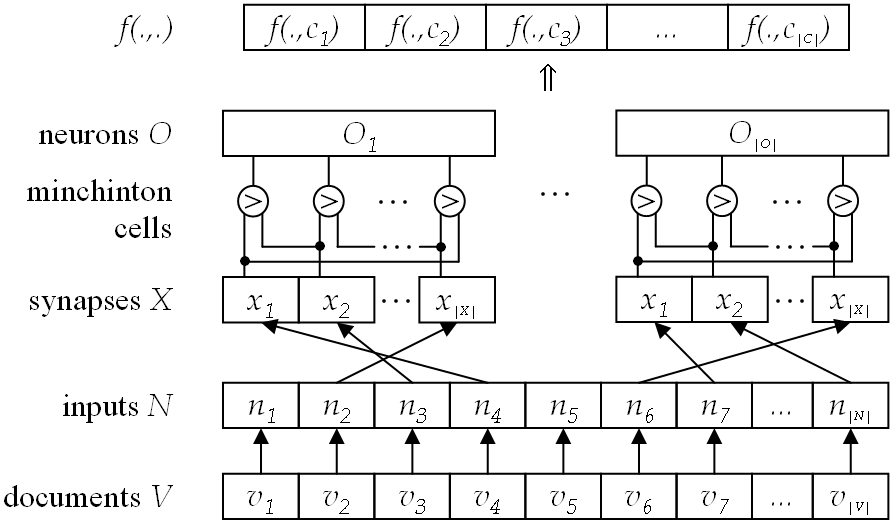
\includegraphics[width=0.6\textwidth]{imagens/arquitetura}
        \end{center}
    \end{figure}
\end{frame}
\begin{frame}
    \frametitle{Exemplo da VG-RAM}
    VG-RAM de 6 bits e $d = 2$
    \begin{table}
        \centering
        \begin{tabular}{|c|c|}
            \hline
            input & output\\
            \hline
        \end{tabular}
    \end{table}
\end{frame}
\begin{frame}
    \frametitle{Exemplo da VG-RAM}
    Valor de treino 100011 associado a 1:
    \begin{table}
        \centering
        \begin{tabular}{|c|c|}
            \hline
             input &   output\\
            \hline
            100011 & \alert 1\\
            \hline
        \end{tabular}
    \end{table}
\end{frame}
\begin{frame}
    \frametitle{Exemplo da VG-RAM}
    Propagação para distância 1:
    \begin{table}
        \centering
        \begin{tabular}{|c|c|}
            \hline
            input &   output\\
            \hline
            000011 & \alert 1\\
            \hline
            100001 & \alert 1\\
            \hline
            100010 & \alert 1\\
            \hline
            100011 &        1\\
            \hline
            100111 & \alert 1\\
            \hline
            101011 & \alert 1\\
            \hline
            110011 & \alert 1\\
            \hline
        \end{tabular}
    \end{table}
\end{frame}
\begin{frame}
    \frametitle{Exemplo da VG-RAM}
    Propagação para distância 2:
    \begin{table}
        \tiny
        \centering
        \begin{tabular}{|c|c|}
            \hline
            input &   output\\
            \hline
            000001 & \alert 1\\
            \hline
            000010 & \alert 1\\
            \hline
            000011 &        1\\
            \hline
            000111 & \alert 1\\
            \hline
            001011 & \alert 1\\
            \hline
            010011 & \alert 1\\
            \hline
            100000 & \alert 1\\
            \hline
            100001 &        1\\
            \hline
            100010 &        1\\
            \hline
            100011 &        1\\
            \hline
            100101 & \alert 1\\
            \hline
            100110 & \alert 1\\
            \hline
            100111 &        1\\
            \hline
            101001 & \alert 1\\
            \hline
            101010 & \alert 1\\
            \hline
            101011 &        1\\
            \hline
            101111 & \alert 1\\
            \hline
            110001 & \alert 1\\
            \hline
            110010 & \alert 1\\
            \hline
            110011 &        1\\
            \hline
            110111 & \alert 1\\
            \hline
            111011 & \alert 1\\
            \hline
        \end{tabular}
    \end{table}
\end{frame}
\end{document}
